\documentclass[11pt]{article}
\usepackage[margin=1in]{geometry}
\usepackage[T1]{fontenc}
\usepackage{lmodern}
\usepackage{amsmath,amssymb,amsthm}
\usepackage{graphicx}
\usepackage[hidelinks]{hyperref}
\usepackage{microtype}
\raggedright

\newtheorem*{theorem}{Theorem}
\newtheorem*{lemma}{Lemma}
\newcommand{\R}{\mathbb R}
\newcommand{\Z}{\mathbb Z}

\begin{document}

\begin{center}
{\Large Partial result for arXiv:1301.5895}\\[4pt]
{\large The covering-pessimum conjecture for two ranges of superballs}
\end{center}

\paragraph{Status.}
\textbf{partial result.}  We prove the source's global conjecture throughout
two infinite subfamilies of three-dimensional superballs.  The result is not
claimed for arbitrary symmetric bodies, and a middle exponent interval remains.

\paragraph{Source conjecture.}
Kallus proves that the Euclidean ball is a strict local maximum of lattice
covering density among origin-symmetric bodies and ends with the following
global conjecture:
\begin{center}
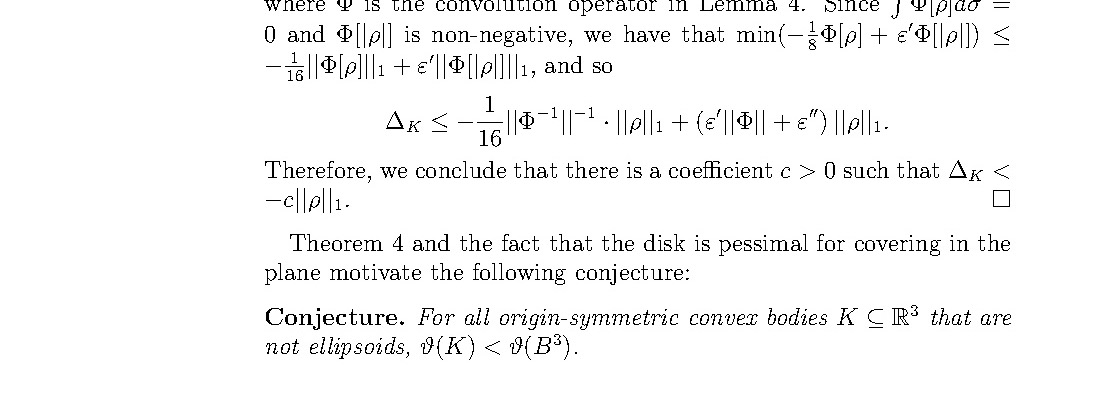
\includegraphics[width=.94\linewidth]{figures/source_conjecture.jpg}
\end{center}

For $1\le p<\infty$, put
\[
 B_p^3=\left\{x\in\R^3:\sum_{i=1}^3|x_i|^p\le1\right\},\qquad
 v_p=\operatorname{vol}(B_p^3)
 =\frac{8\Gamma(1+1/p)^3}{\Gamma(1+3/p)}.
\]
The Euclidean ball has optimal lattice covering density
\[
 \vartheta(B_2^3)=\frac{5\sqrt5\,\pi}{24}=1.463503\ldots .
\]

\begin{theorem}
For every $1\le p<2$ and every $p\ge9$,
\[
 \vartheta(B_p^3)<\vartheta(B_2^3).
\]
At $p=2$ equality holds, as all ellipsoids are affine images of the ball.
\end{theorem}

\section*{The BCC certificate for $1\le p\le2$}

Let
\[
 \Lambda_{\rm BCC}=\Z^3\cup\bigl(\Z^3+h\bigr),
 \qquad h=(1/2,1/2,1/2).
\]
It is a lattice of determinant $1/2$.

\begin{lemma}
For every $p\ge1$, the $\ell_p$ covering radius of
$\Lambda_{\rm BCC}$ is exactly
\[
 r_p=\frac12\bigl(1+2^{-p}\bigr)^{1/p}.
\]
\end{lemma}

\begin{proof}
Reduce a point modulo $\Z^3$ and reflect its coordinates.  Reflections preserve
both cosets, so the point is represented by $z/2$ with $z\in[0,1]^3$.
Its distance to the lattice is at most
\[
 \frac12\min\left\{
   \left(\sum z_i^p\right)^{1/p},
   \left(\sum(1-z_i)^p\right)^{1/p}
 \right\}.
\]
At least one of $\sum z_i$ and $\sum(1-z_i)$ is at most $3/2$.
The convex function $\sum z_i^p$ attains its maximum on
$\{z\in[0,1]^3:\sum z_i\le3/2\}$ at an extreme point; the largest value is
$1+2^{-p}$, attained at permutations of $(1,1/2,0)$.  This proves the upper
bound.  At $z=(1,1/2,0)$, coordinatewise nearest-point inspection in both
cosets shows that the displayed two distances are equal to $r_p$ and no other
lattice point is closer.  Hence the bound is exact.
\end{proof}

The corresponding covering density is
\begin{equation}\label{bccdensity}
 D_{\rm BCC}(p)
 =\frac{v_pr_p^3}{\det\Lambda_{\rm BCC}}
 =\frac{v_p}{4}\bigl(1+2^{-p}\bigr)^{3/p}.
\end{equation}

\begin{lemma}
$D_{\rm BCC}(p)$ is strictly increasing on $1\le p\le2$.
\end{lemma}

\begin{proof}
Set $t=1/p$, $a=2^{-1/t}$, and differentiate the logarithm of
\eqref{bccdensity}.  With $\psi=\Gamma'/\Gamma$ one obtains
\[
 \frac13\frac{d}{dt}\log D_{\rm BCC}(1/t)
 =\psi(1+t)-\psi(1+3t)+R(t),
\quad
 R(t)=\log(1+a)+\frac{a\log2}{t(1+a)}.
\]
The series for the trigamma function and comparison with its integral give
\[
 \psi(1+3t)-\psi(1+t)
 =\int_{1+t}^{1+3t}\psi'(u)\,du
 >\log\frac{1+3t}{1+t}.
\]
It remains to check $H(t):=\log\frac{1+3t}{1+t}-R(t)>0$ on
$[1/2,1]$.  Differentiation gives
\[
 H'(t)=\frac{2}{(1+t)(1+3t)}
 -\frac{(\log2)^2a}{t^3(1+a)^2},
\]
whose sign is the sign of
\[
 Q(t)=2t^3(1+a)^2-(\log2)^2a(1+t)(1+3t).
\]
Direct differentiation shows $Q'(t)>0$ on $[1/2,1]$.
Moreover $Q(.55)<0<Q(.56)$, $H(.55)>.0082$, $H(.56)>.0081$, and on
$[.55,.56]$, monotonicity of the two terms gives
\[
 H(t)\ge
 \log\frac{1+3(.55)}{1+.55}-R(.56)>.0033.
\]
Thus $H>0$.  The decimal inequalities are certified by directed interval
arithmetic in the included verifier (which also certifies $Q'>0$ on 5,000
subintervals); they merely abbreviate an elementary one-variable check.
Therefore the displayed logarithmic derivative is negative, which is
equivalent to strict increase in $p$.
\end{proof}

At $p=2$, formula~\eqref{bccdensity} becomes exactly
\[
 \frac{4\pi/3}{4}\left(1+\frac14\right)^{3/2}
 =\frac{5\sqrt5\,\pi}{24}.
\]
The monotonicity lemma proves the theorem for $1\le p<2$.

\section*{The cubic certificate for $p\ge9$}

The covering radius of $\Z^3$ in $\ell_p^3$ is
$3^{1/p}/2$, attained at the center of its unit cube.  Hence
\[
 \vartheta(B_p^3)
 \le \frac{v_p3^{3/p}}8
 \le 3^{3/p},
\]
because $B_p^3\subset[-1,1]^3$ and therefore $v_p\le8$.
For $p\ge9$ this is at most $3^{1/3}<1.443$, whereas
\[
 \frac{5\sqrt5\,\pi}{24}
 >\frac{5(2.236)(3.1415)}{24}>1.4634.
\]
This proves the second range.

\section*{Upgrade audit and limitations}

Eight focused attacks are detailed in the accompanying attempt note.  In
particular, exact boundary checks show why the BCC lattice ceases to certify
the result for $p>2$: the witness $(1,1/2,0)$ persists and its density rises
above the ball value.  A rhombohedral numerical search initially looked
better, but auditing its faces exposed omitted covering holes.  Cubic and
planar-product lattices also leave a gap.

Thus this packet does not settle $2<p<9$, arbitrary origin-symmetric bodies,
or the full global conjecture.  The source's local theorem does cover some
unspecified neighborhood of $p=2$; the new contribution here is a global
certificate along the whole lower superball branch and an elementary far-end
certificate on the upper branch.

\paragraph{Verification.}
The exact cell argument is independent of computation.  The included script
provides directed-interval certification of the only scalar calculus lemma,
checks half a million cell points and all equality witnesses used by the
formula, and verifies density sanity values.  A bounded title/exact-conjecture
search found no later full resolution.

\begin{thebibliography}{9}
\bibitem{Kallus}
Y. Kallus,
\emph{When is the ball a local pessimum for covering?},
Discrete Comput. Geom. \textbf{54} (2015), 232--245;
arXiv:1301.5895.
\end{thebibliography}

\end{document}
